\begin{frame}[fragile]{fragmentation}
\begin{itemize}
\item max frame data size on my local network = 1500 bytes, but\ldots
\end{itemize}
\begin{Verbatim}
$ ping6 fe80::da07:b6ff:fed9:ae50 -s 4000
PING fe80::da07:b6ff:fed9:ae50 (fe80::da07:b6ff:fed9:ae50) 4000 data bytes
4008 bytes from fe80::da07:b6ff:fed9:ae50%eno1: icmp_seq=1 ttl=64 time=1.17 ms
4008 bytes from fe80::da07:b6ff:fed9:ae50%eno1: icmp_seq=2 ttl=64 time=0.779 ms
4008 bytes from fe80::da07:b6ff:fed9:ae50%eno1: icmp_seq=3 ttl=64 time=0.742 ms
...
$ ping -s 4000 192.168.1.1                 
PING 192.168.1.1 (192.168.1.1) 4000(4028) bytes of data.     
4008 bytes from 192.168.1.1: icmp_seq=1 ttl=64 time=0.891 ms 
4008 bytes from 192.168.1.1: icmp_seq=2 ttl=64 time=0.806 ms 
4008 bytes from 192.168.1.1: icmp_seq=3 ttl=64 time=0.748 ms 
\end{Verbatim}
\end{frame}

\begin{frame}{IPv6 fragments}
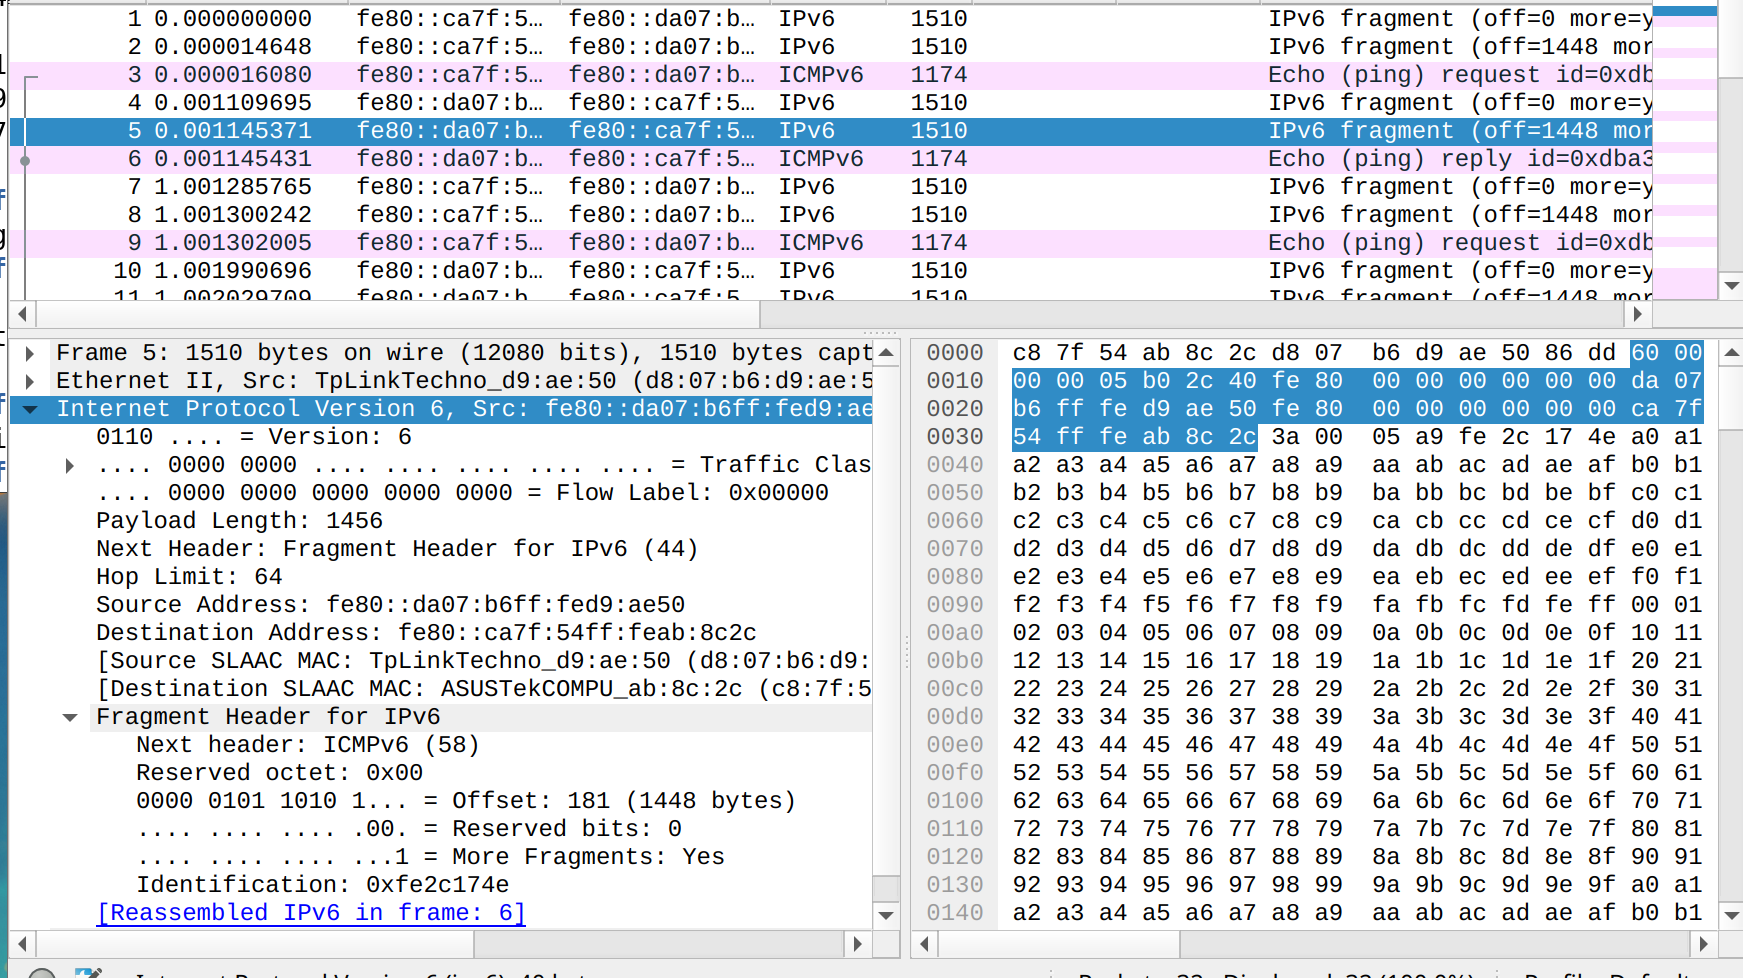
\includegraphics[width=\textwidth]{../routing/ipv6-fragment-ex}
\end{frame}

\begin{frame}{IPv4 fragments}
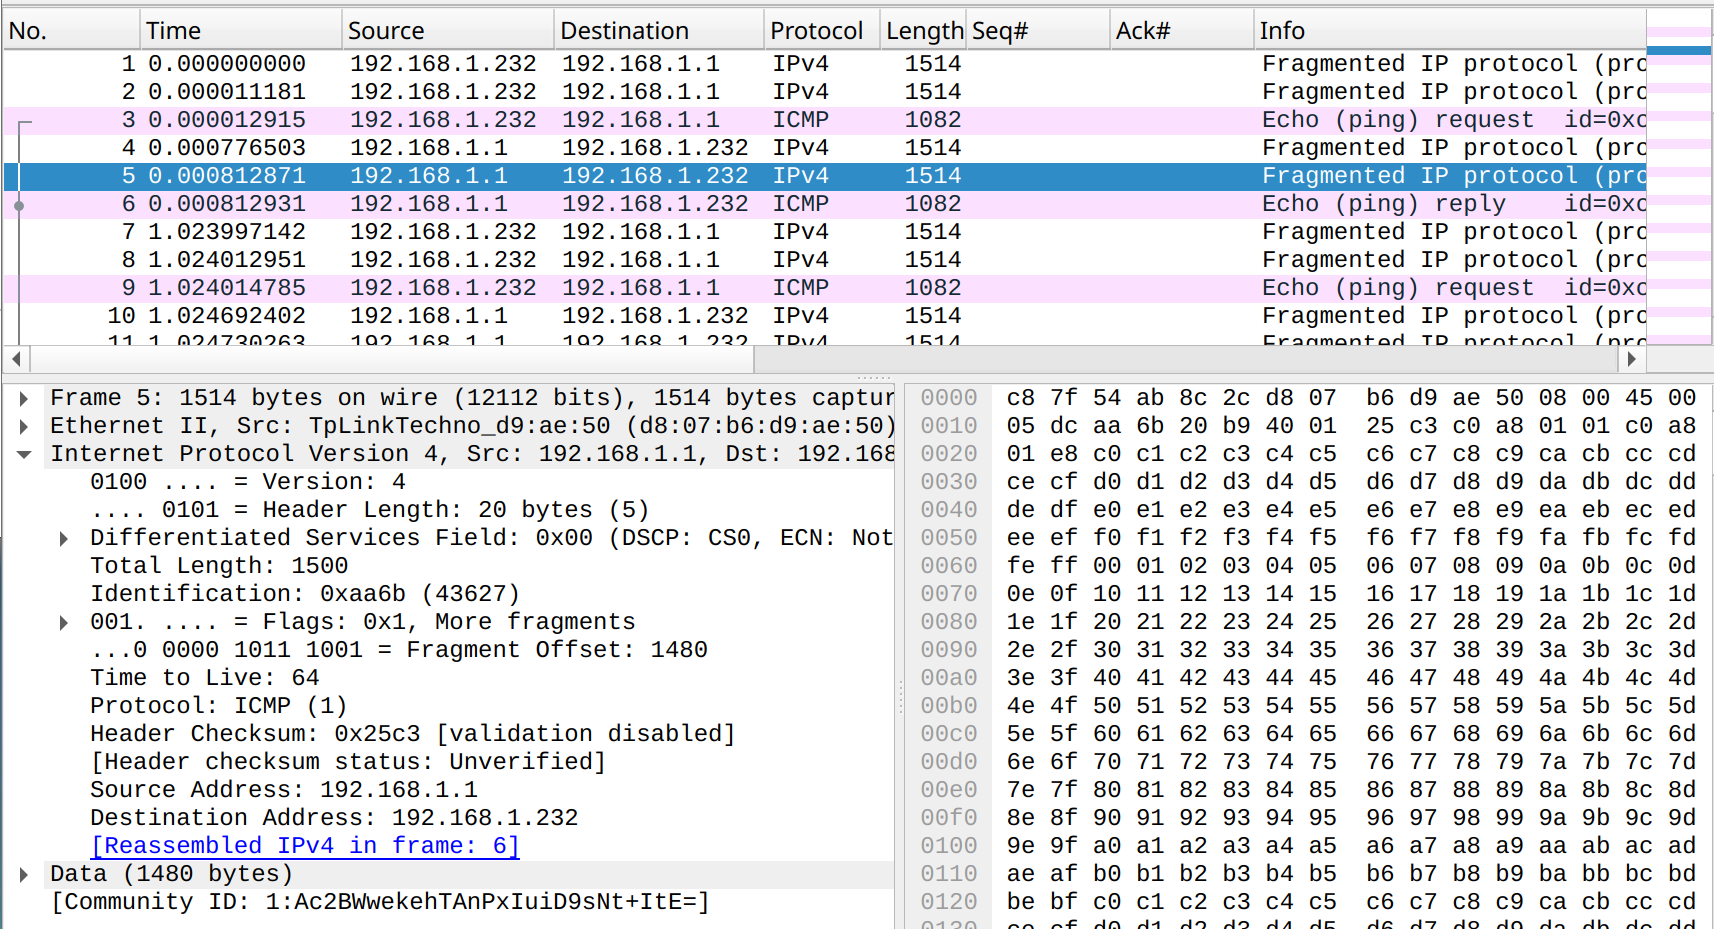
\includegraphics[width=\textwidth]{../routing/ipv4-fragment-ex}
\end{frame}

\begin{frame}{varying frame size support}
    \begin{itemize}
    \item also called \textit{maximum transmission unit} (MTU)
    \vspace{.5cm}
    \item typical Ethernet, Wifi --- 1500 bytes
    \item Ethernet with ``jumbo frames'' -- 65535 bytes
    \item IPsec ESP VPN over 1500-byte MTU network -- $\sim$1400--1440 bytes
        \begin{itemize}
        \item VPN --- simulated network link over other network links
        \end{itemize}
    \end{itemize}
\end{frame}

\begin{frame}{routers making fragments}
    \begin{itemize}
    \item option in IPv4 to handle frame size mismatch, but not great:
    \vspace{.5cm}
    \item extra data sent over network (especially if just over max size)
        \begin{itemize}
        \item extra copies of main headers on each fragment
        \end{itemize}
    \item extra work at receiver to reconstruct fragments
    \item lose whole packet if one fragment is lost
        \begin{itemize}
        \item but other routers likely to still waste time forwarding all other fragments
        \end{itemize}
    \end{itemize}
\end{frame}

\begin{frame}{avoiding fragmentation}
    \begin{itemize}
    \item IPv4 --- DF (don't fragment) flag in packets
        \begin{itemize}
        \item if set, routers not allowed to fragment packet
        \end{itemize}
    \item IPv6 --- routers never fragment packets
        \begin{itemize}
        \item any fragments made at source machine only
        \end{itemize}
    \vspace{.5cm}
    \item<2-> when set --- ICMP error
        \begin{itemize}
        \item ICMPv6: Packet Too Big
        \item ICMPv4: destination unreachable + reason code of fragmentation needed
        \item (hopefully, bad networks might drop packet instead)
        \end{itemize}
    \item<2-> ICMPv6 error tells you maximum supported size
        \begin{itemize}
        \item (by first link that got packet rejected --- might be more constraining link later)
        \item info not available in IPv4
        \end{itemize}
    \end{itemize}
\end{frame}
